\section{Results}

Following the methodology described in the previous section, we estimate the total U.S. Resource to be 3700 $\pm$400 TWh/yr (Table~\ref{table:totals}). Nearly two-thirds of this is in Alaska where a large resource area and energetic waves in the North Pacific combine to create a large total (2000 - 2550 TWh/yr). The U.S. West Coast has a large remote resource (420 TWh/yr) where energetic waves from the North Pacific arrive from offshore.  The West Coast natural local resource is modest in comparison (90 TWh/yr), but there is potentially another 210 TWh/yr available in the potential resource.

The U.S. East Coast resource, on the other hand, is composed primarily of the local resource (180-230 TWh/yr) and has a relatively modest remote portion (110 TWh/yr). This is because mid-latitude westerly winds tend to generate wave energy that propagates eastward, and relatively less wave energy from the open ocean propagates onshore from the open ocean (i.e., compared to the West Coast). This also indicates that much of the East Coast wave resource is located farther from shore, where there is sufficient fetch to have generated the wave energy. \note{Is that last sentence accurate? Assuming yes, is a citation needed for that or is it `simple physics'-enough to simply be stated?}

Hawaii has a large resource due largely to waves that arrive from the North Pacific along the northern boundary of the EEZ surrounding the islands. The natural local resource is relatively small, due primarily to the fact that the sea-state in this region is -- in the long-average perspective presented here, and compared to regions such as the East Coast where wave growth dominates, or compared to the `potential' case -- roughly `steady-state' because the wind input and dissipation are relatively balanced. The Caribbean region (Gulf of Mexico, Puerto Rico, and U.S. Virgin Islands) on the other hand, has a modest wave resource composed predominantly of local wind input. \note{Is ``the Caribbean region'' a term, or is there something better I should use?} The remote resource of this region is also very small because the majority of the U.S. EEZ boundary throughout this region borders other EEZs (rather than being exposed to the open ocean), and the methodology described here only counts wave energy crossing into the EEZ from the open-ocean.

\begin{table}[ht]
  \centering
  \begin{tabular}{|c|c|c|c|c|c|}
    \cline{2-6}
    %\multirow{1}{*}{Region}
    \multicolumn{1}{c|}{} & {\it EPRI 2011} & \multicolumn{4}{c|}{New} \\
    \hline
    Region & Remote  & Remote & \multicolumn{2}{c|}{Local} & Total \\
    & & & Natural & Potential & \\
    \hline
    Alaska & 1570 & 1040 & 990 & 1510 & 2030 - 2550 \\
    West Coast & 590 & 420 & 90 & 210 & 510 - 630 \\
    Hawaii & 130 & 370 & 10 & 100 & 380 - 470 \\
    East Coast & 240 & 110 & 180 & 230 & 290 - 340 \\
    Gulf of Mexico & 80 & 13 & 56 & 57 & 69-70 \\
    P.R. \& U.S.V.I. & 30 & 6 & 11 & 27 & 17 - 33 \\
    \hline \hline
U.S. TOTAL & 2640 & 1960 & 1340 & 2130 & 3300 - 4090 \\
\hline
  \end{tabular}
  \caption{Wave resource assessment results by region and totaled for the entire U.S. (all values in TWh/yr). The range in the total column indicates the sum of Remote+Local (lower value) and Remote+Potential (higher value). \note{Do we need to be more careful w/ significant digits here?}}
  \label{table:totals}
\end{table}

\subsection{Comparison to previous results}
\note{Argh! I'm struggling with how to organize this section! What is the point of all this?}

% This is nearly double the total U.S. wave resource estimated in EPRI 2011. This result is due primarily to two mutually supportive changes to the methodology: 1) the extension of the assessment to the edge of the EEZ, and 2) the inclusion of the local resource in the total. 
% The third fundamental change in the methodology -- utilizing a one-way dot-product -- actually reduces the resource estimates compared to EPRI 2011, but that change is overwhelmed by the increases due to the other changes.

Our estimate of the total wave energy resource is 25-50\% larger than the EPRI 2011 assessment. This result, however, should not be interpreted too strongly because the majority of this increase is due to including the ``local resource'' over the vast U.S. EEZ, and it is unclear whether this is a technically viable resource. That is, while the energy is theoretically available and contained within U.S. maritime boundaries it is likely to be especially technically challenging to harness.

A more pragmatic comparison is to compare the EPRI 2011 results to the inner-shelf results presented in table \ref{tab:nearshore-total}. Here the ``inner-shelf'' results are computed following the same methodology as described in section \ref{sec:method}, but we use the 10-nm boundary as the integration contour for all regions. This is a closer comparison to the EPRI 2011 results because it is comparable to the location of the 200-m depth contour in most regions. \note{Should we use the 30-nm boundary, or the 50-nm boundary for this? If so, should we not include the local resource in this comparison? What is the point of comparing the results?!} 

Rather,  is due primarily to the inclusion of the local resource term, which was not included in EPRI 2011, and to the fact that this analysis has been extended to include the entire EEZ. 
There are three important pieces of the EPRI 2011 methodology that are different from what is used here:
\begin{enumerate}
\item It includes only the remote resource, because the local resource was not typically considered in wave energy resource assessment at that time
\item It used an integration contour that was much closer to shore (i.e., the 200-m water-depth contour, or 50 nautical-miles from shore, whichever is closer to shore)
\item It did not account for wave directionality, which led to some ``double-counting'' \cite{nationalresearchcouncilEvaluationDepartmentEnergy2013}
\end{enumerate}

did not include any estimate of the `pointing out that the new ``remote'' results are lower than the EPRI 2011 results (which estimated the remote resource only) for all regions except Hawaii (Table~\ref{table:totals}). The Hawaii resource is the exception because we utilize the EEZ surrounding the State's islands rather than the 200-m isobath used in the EPRI 2011 results (i.e., we are casting a much wider net). Alaska and the West Coast are reduced by approximately 30\%, which can be attributed primarily to accounting for wave directionality. The east coast, Gulf of Mexico, and caribbean island territories are reduced by 55-80\% for two reasons: 1) accounting for directionality, and 2) the integration contour used for these regions is significantly shorter than that used in EPRI 2011, primarily because large portions of the U.S. EEZ boundary in this region is a ``border'' with another country's EEZ. All together, the total remote resource estimated here is 25\% smaller than the EPRI 2011 estimate.

Adding the local resource to the total changes the story completely. The magnitude of the local resource for most regions is comparable to the remote resource. The potential resource (local resource without remote waves) is larger than the remote resource for all regions except Hawaii and the West Coast.

%The inclusion of the local resource is especially important because without it, we would be comparing the new remote results with the EPRI 2011 results, (be left to compare the  methodological change (relative to EPRI 2011): accounting for wave directionality, delivers a significant reduction in the total resource across all regions

In order to understand the source of these changes, we begin by noting that -- except for Hawaii -- the new remote results are much {\em lower} than the EPRI 2011 results. This is due to accounting for wave-directionality (using a one-way dot-product). Hawaii is the exception because by extending the analysis to the edge of the EEZ, we have cast a much wider net than was used in EPRI 2011 (which utilized the 200-m isobath as the integration contour) and this overwhelms the reduction of resource due to directionality. The other regions, however, do not enjoy a longer integration contour and therefore accounting for directionality reduces the resource total by more than 30\%. The regions that see the largest reductions in remote resource (e.g., the Gulf of Mexico) were further reduced by the fact that the majority of the EEZ boundary in these regions are `borders' with other nations, and therefore the integration contour in these regions is much shorter than was utilized in EPRI 2011.

So, we now have a solid methodology for estimating the remote resource that is in broad agreement with several previous works, even if the results are somewhat dissappointing compared with the now debunked EPRI 2011 results. Furthermore, it should be noted that the `new remote' values are in good agreement with EPRI 2004 results, which utilized essentially an identical methodology as used here to estimate the remote resource (see EPRI 2011 for EPRI 2004 results).
% I can't find the EPRI 2004 paper online anymore!? Ask Hagerman for this (it isn't cited in 2011 report either)!


EPRI 2011, the 200-m depth contour that was used was much shorter the extension of theThis is primarily due to a comHere we see that the new results are more than 30\% lower than the EPRI 2011 results.
% These two quantities are similar in that they both do not include the local resource, but they are still based on fundamentally different methods: 1) the new remote results are based on a one-way vector line-integral, rather than the now debunked ``unit-circle method'', and 2) the new results use the edge of the EEZ as the integration contour, while the EPRI 2011 results utilized the 200-m depth contour (or 50 nautical miles from shore, whichever is closer to shore). These methodological differences cause distinct regional changes in the resource magnitude.

On the U.S. West and East Coasts, and in Alaska, the new remote resource is 30-55\% lower than the EPRI estimate primarily due to accounting for wave directionality. This drop is particularly pronounced on the East Coast for two reasons:
\begin{enumerate}
\item because more of the wave energy there is propagating offshore, which is not included in the one-way dot-product (note, however, that the energy which originates from within the U.S. EEZ and propagates offshore {\em is counted} as part of the local resource). 
\item The length of the contour decreases (i.e., most of the FL coastline isn't counted) because it borders other EEZs? \note{Need to check this?}
\end{enumerate}
The Gulf of Mexico, Puerto Rico, and U.S. Virgin Islands 

\note{Do we also need to mention minor differences in method: different model and duration?} The first of these changes leads to a reduction in total resource, while the second changes the result in proportion to the change in the length of the contour.

The EPRI 2011 assessment had three distinct differences from the current approach: 1) it computed only the remote resource, 2) it did so along the 100-m isobath, and 3) it utilized a 'unit-circle' line-integral method that was critiqued for `double-counting'. 
the revised methodology proposed herein, which is focused primarily on establishing a consistent and comprehensive methodology, rather than a fundamentally new understanding of wave physics. In other words, this work has not ``discovered new wave energy'', so much as modified the methodology to account for the wave energy potential over the entirety of the U.S.'s EEZ.

This increase is a result of changes to the methodology we've proposed. On one hand, 
but most of this increase is due to adding the local resource over the U.S. EEZ to the total, which was not included in the EPRI 2011 assessment. 


The EPRI 2011 resource assessment was different from this work in three important ways:
\begin{itemize}
\item It did not account for wave directionality.
\item It computed the wave resource along the 100m isobath, rather than the full EEZ.
\item It did not account for the local resource.
\end{itemize}


\note{Need to work on this...}
The large increase in resource in Hawaii is due in large part due to the exteneded area of integration. In the EPRI 2011 report the integration was performed at the 200 m isobath, which in the case of Hawaii is very close to shore due to the lack of continental shelf. In the present case, integration contour is extented to the EEZ which lies at 200 nmi in the Northern, Eastern, and Southern boundaries.

\begin{table}[ht]
  \centering
  \begin{tabular}{|c|c|c|}
    \hline
    Region & EPRI 2011 &Inner-Shelf Resource \\
    \hline
    Alaska & 1570 &1100 \\
    West Coast & 590 & 410 \\
    Hawaii & 130 & 120 \\
    East Coast & 240 & 90 \\
    Gulf of Mexico & 80 & 20 \\
    P.R. \& U.S.V.I. & 30 & 20 \\
    \hline \hline
    U.S. TOTAL & 2640 & 1800 \\
    \hline
  \end{tabular}
  \caption{Inner-shelf resource. \note{Do we want/need to include this? It probably belongs in a different table? Or does it make sense on it's own like this?}}
  \label{tab:nearshore-total}
\end{table}

\subsection{Wave energy distribution within each region}

\begin{figure}[ht]
  \centering
  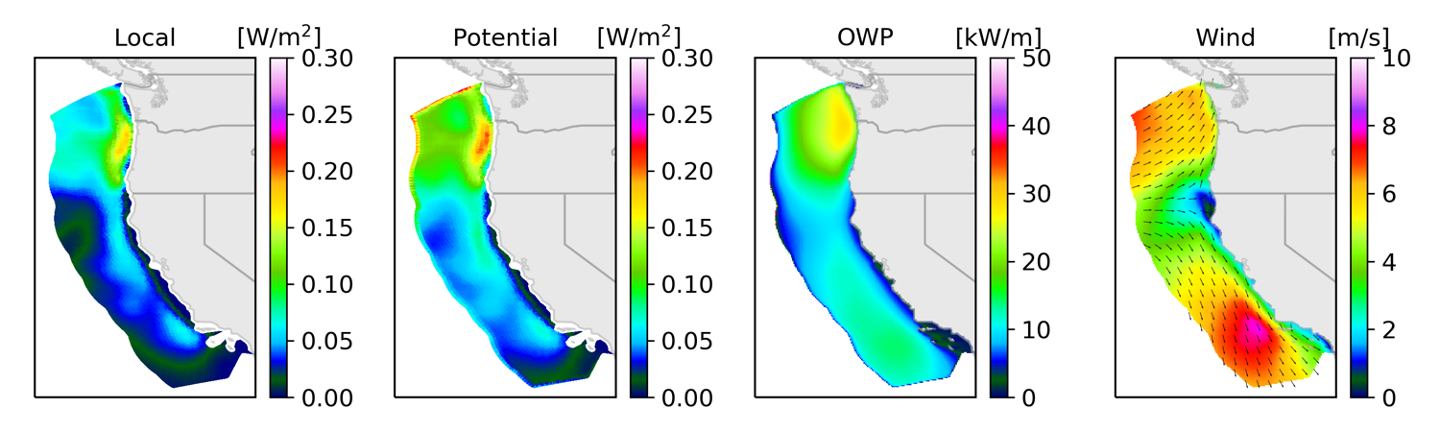
\includegraphics[width=\textwidth]{../fig/WC-Map01-November.png}
  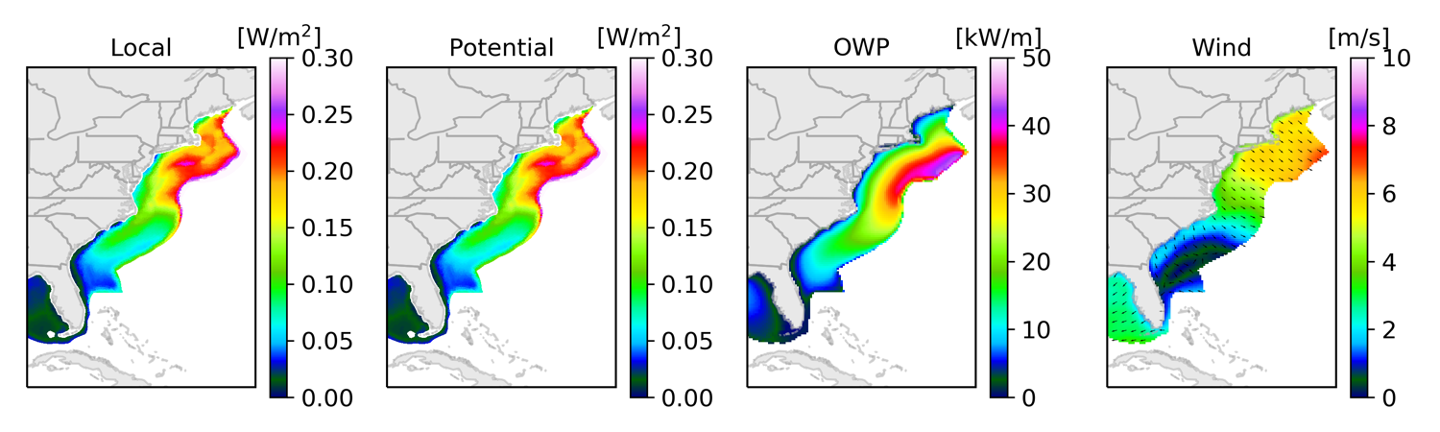
\includegraphics[width=\textwidth]{../fig/EC-Map01-November.png}
  \caption{Maps of wave resource for the West Coast (top), and East Coast (bottom). \note{GGM: Can we get these as total annual averages, or are those `boring'? Can we add mean wave-direction to the OWP plot?}}
  \label{fig:maps}
\end{figure}

\note{GGM: Regarding Figure \ref{fig:maps}: why are winds and 'potential resource' so different on WC? I would think they would be more spatially correlated? Specifically: why is wind high off of S. Cali, but potential/local resource is highest offshore of OR/WA? ... I think you've answered this question before, but I forget.}

Do we want these plots?
\begin{itemize}
\item Plots of ‘remote’ resource vs. distance from shore (Figure 5). ... How does this compare with local resource vs. distance from shore?
\item Remote resource vs. depth. Local resource vs. depth.
\end{itemize}

\subsection{Annual cycle of wave energy resource}

The annual cycle of the wave energy resource has a remarkably consistent pattern across all U.S. regions (Figure \ref{fig:annual-cycle}). Wave energy is a late-fall and winter dominated resource. The resource peaks in December or January across all regions, and is at a minimum in summer months. The inter-annual variability of the monthly-averaged West Coast resource is small during summer months when the resource is small (Figure \ref{fig:wc-variability}). During energetic winter months, the monthly-averaged resource can vary by more than 50\%, but in general the interannual variability is less than 30\% of the month's mean. This suggests that during energetic winter months wave energy projects should be expected to deliver at least their annual mean, with the potential of providing up to three-times that value. \note{Is that last sentence a stretch? Am I glossing over too many details about site-specific variability and device performance characteristics?} However, more detailed analysis is required to demonstrate these characteristics at individual sites and for individual technologies. Other regions have similar variability characteristics (not shown for simplicity).

\begin{figure}[ht]
  \centering
  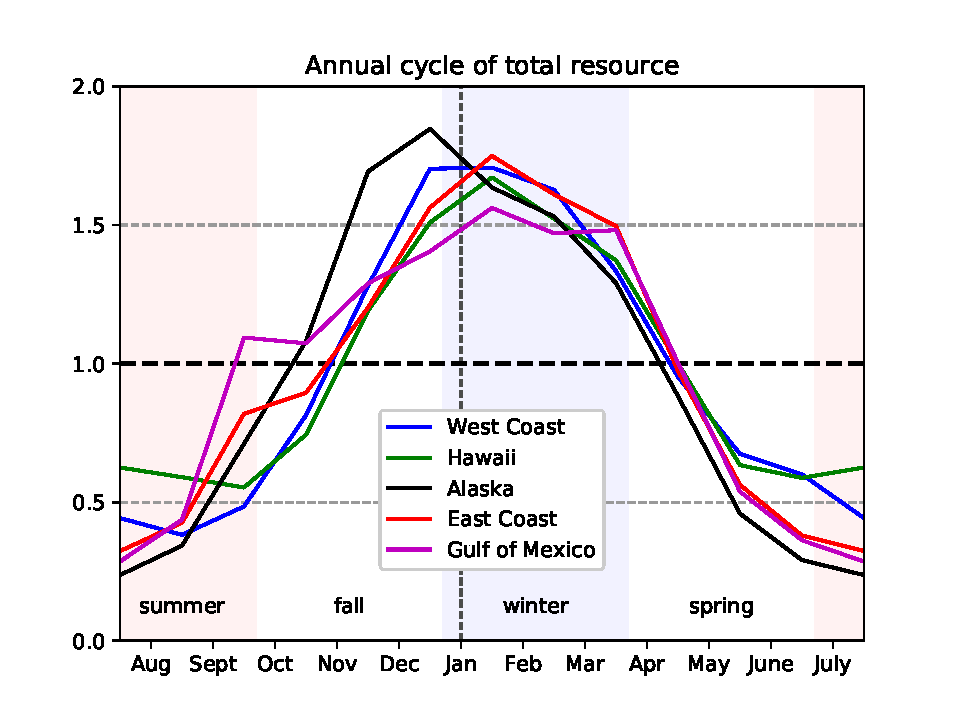
\includegraphics[width=\textwidth]{../fig/AnnualCycle01.pdf}
  \caption[Wave resource annual cycle.]{The annual cycle of the total wave energy resource for several regions, relative to the regional mean.}
  \label{fig:annual-cycle}
\end{figure}


\begin{figure}[ht]
  \centering
  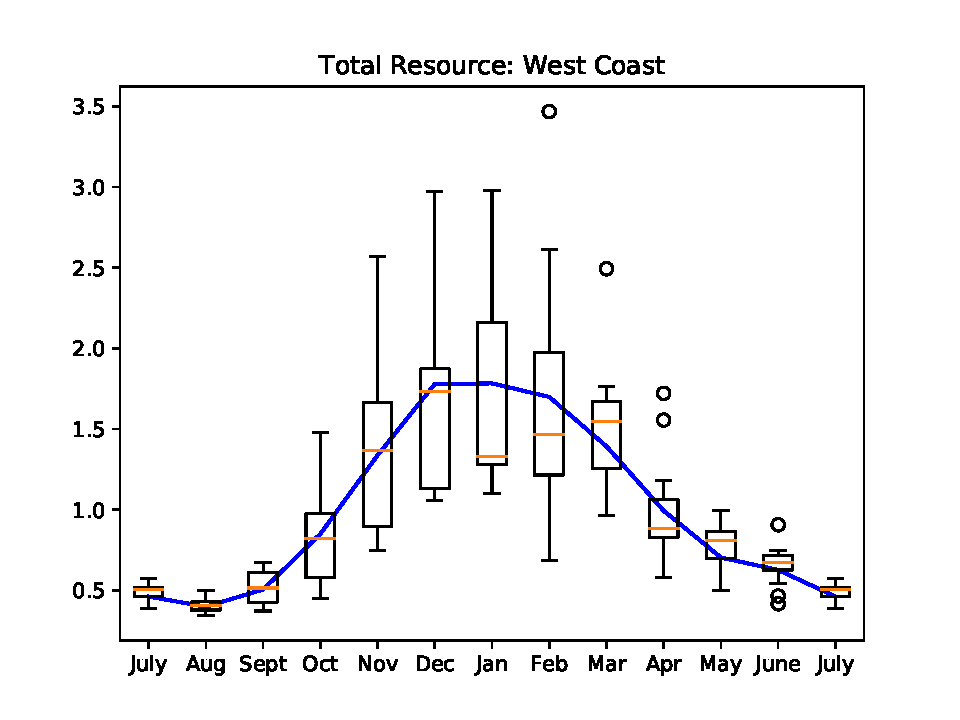
\includegraphics[width=\textwidth]{../fig/AnnualVar01.wc.pdf}
  \caption[West Coast resource variability.]{Annual and inter-annual variability of the West Coast resource. The thick solid line indicates the mean, and the orange lines and boxes indicate the median and quartiles, respectively. The whiskers extend to the last point within 1.5x of the inter-quartile range, and points beyond this are plotted as open-circles.}
  \label{fig:wc-variability}
\end{figure}

\subsection{Frequency dependence of wave resource}

\begin{figure}[ht]
  \centering
  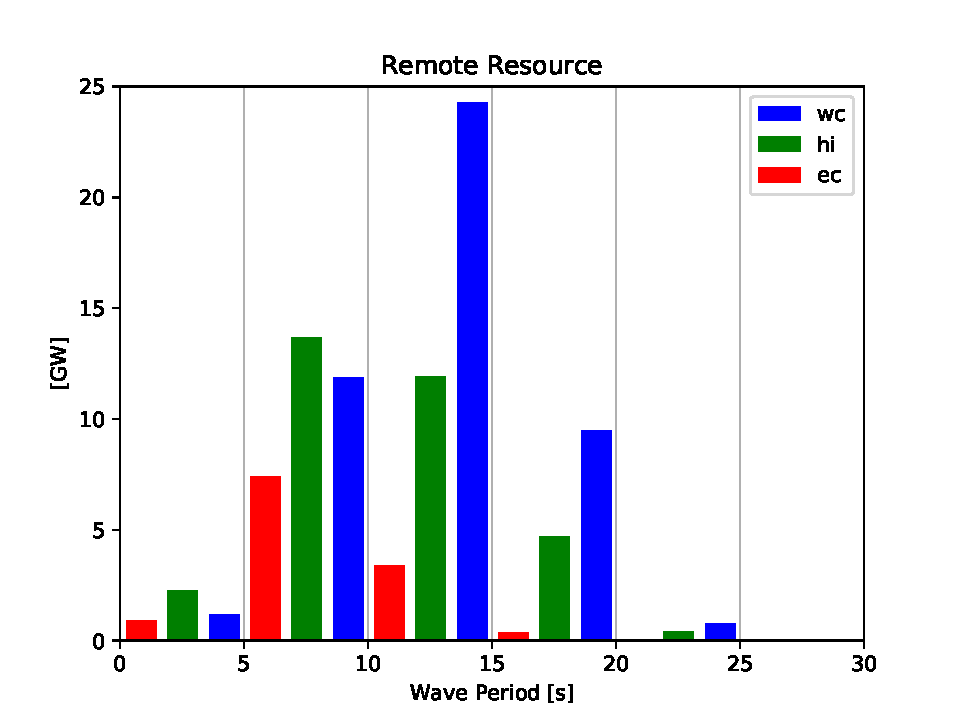
\includegraphics[width=\linewidth]{../fig/RemoteResource_Freq01.pdf}
  \caption{Remote resource contained in each wave period band (0-5 seconds, 5-10 seconds, etc.) for the west coast, Hawaii, and the east coast.}
  \label{fig:remote-freq}
\end{figure}

\begin{figure}[ht]
  \centering
  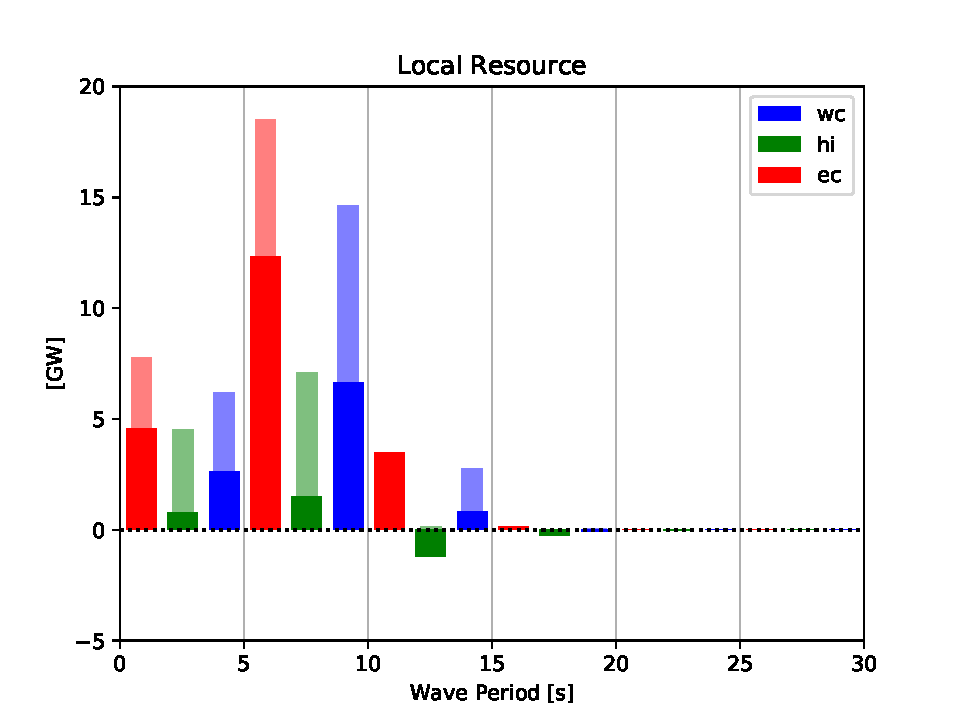
\includegraphics[width=\linewidth]{../fig/LocalResource_Freq01.pdf}
  \caption{Local (thick solid bars) and potential (narrow pale bars) resource contained in each wave period band (0-5 seconds, 5-10 seconds, etc.) for the west coast (wc), Hawaii (hi), and the east coast (ec).}
  \label{fig:remote-freq}
\end{figure}

\begin{itemize}
\item Regional differences in frequency dependence?
\item Frequency dependence of local vs. remote?
I don't think we're adding these any more?
\end{itemize}


%%% Local Variables:
%%% TeX-master: "wave_res"
%%% End:
